\documentclass[10pt]{article}
\usepackage[polish]{babel}
\usepackage[utf8]{inputenc}
\usepackage[T1]{fontenc}
\usepackage{amsmath}
\usepackage{amsfonts}
\usepackage{amssymb}
\usepackage[version=4]{mhchem}
\usepackage{stmaryrd}
\usepackage{graphicx}
\usepackage[export]{adjustbox}
\graphicspath{ {./images/} }

\title{GIMNAZJUM }

\author{}
\date{}


\begin{document}
\maketitle
\begin{enumerate}
  \item Rozstrzygnij, czy można liczby \(1,2,3, \ldots, 18\) rozstawić w wierzchołkach i na środkach krawędzi ośmiościanu foremnego tak, aby każda liczba leżąca na krawędzi ośmiościanu była średnią arytmetyczną liczb leżących na jej końcach.
  \item Wyznacz wszystkie liczby naturalne \(a, b\), aby liczba \(n\) spełniająca równanie też była naturalna.
\end{enumerate}

\[
\frac{1}{a}+\frac{1}{b}=n
\]

\begin{enumerate}
  \setcounter{enumi}{2}
  \item Punkt S jest środkiem okręgu wpisanego w trójkąt ABC. Di E są takimi punktami boku AB, że odcinek DS jest równoległy do boku AC, a odcinek ES - do boku BC. Udowodnij, że obwód trójkąta DES jest równy długości odcinka AB.\\
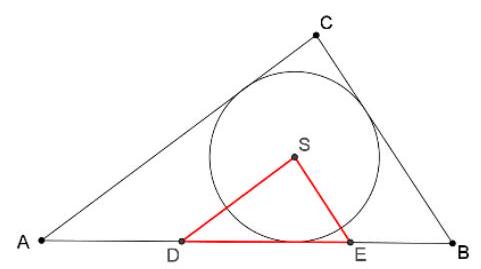
\includegraphics[max width=\textwidth, center]{2024_11_21_9b8ada7da6a3760c69dcg-1}
\end{enumerate}

\section*{LICEUM}
\begin{enumerate}
  \item Współczynniki \(a, b, c, d\) wielomianu \(W(x)=x^{4}+a x^{3}+b x^{2}+c x+d\) są liczbami całkowitymi nieparzystymi. Udowodnij, że wielomian ten nie posiada pierwiastków całkowitych.
  \item Wyznacz wszystkie pary liczb pierwszych \(p, q\) spełniające równanie:
\end{enumerate}

\[
p^{2}-2 q^{2}=1
\]

\begin{enumerate}
  \setcounter{enumi}{2}
  \item Dany jest trapez, w którym suma kątów przy podstawie wynosi \(90^{\circ}\), a ramiona mają długości 15 i 36 . Oblicz długość odcinka łączącego środki podstaw.
\end{enumerate}

\end{document}